\chapter{Introduction}


\section{Cosmology and the cosmic dawn}

\subsection{Modern cosmology and the history of the universe}

Much like particle physics, cosmology today finds itself in the enviable yet frustrating position of having a broadly supported picture of the universe with only the most challenging and fundamental questions unanswered. Many intersecting lines of evidence point to a universe which began hot, dense, homogenous, and rapidly expanding 13.8 billion years ago, eventually cooled enough for bound objects to form, and is now accelerating. Studies of the Cosmic Microwave Background (CMB), high-z supernovae, distant galaxies, primordial element abundances, the matter power spectrum, and other observables all converge on this model. It is largely, however, a mal-understood and entirely unexpected \textit{dark} universe, whose total energy budget is dominated by constituents whose gravitational properties are well understood, but whose fundamental nature remains mysterious. 

The simplest (i.e., \textit{vanilla} model which agrees with all available data is parameterized by the energy densities of baryons ($\Omega_b=0.0455\pm0.0003$), cold dark matter  ($\Omega_m=0.3089\pm0.0062$), and vacuum energy ($\Omega_\Lambda=0.69\pm0.0062$), the amplitude ($\ln (10^{10}A_s)=3.064\pm0.023$) and spectral index ($n_s=0.9667\pm0.004$) of the primordial power spectrum, and the optical depth to reionization ($0.066\pm0.012$). 
The energy densities are given as the present densities of these constituents relative to the present critical density $\rho_c=3H_0^2/8\pi G$, where the present expansion rate is $(70\pm3$)\,km/s/Mpc
\footnote{I've taken the uncertainty on $H_0$ to be the spread between the CMB measurement of $67.74\pm0.46$ km/s/Mpc \citep{planck16} and the local measurement of $73.2\pm1.7$ \citep{reiss16}.}. 
On scales larger than hundreds of Mpc, our universe is flat, deviating from Euclidian geometry only due to a homogenous and isotropic expansion, with a measured curvature density consistent with zero of $\Omega_K=0.008\pm0.004$. 
Further, the equation of state of dark energy is constrained to be $w=-1.02\pm0.08$, consistent with -1, and thus, with a true cosmological constant or a uniform vacuum energy. These measurements represent the best combined constraints reported by \citet{planck16}, and have been made possible by the avalanche of data on the CMB, weak lensing statistics, baryon acoustic oscillations, and type 1a supernova surveys collected in recent years. 

In this framework, the history of the universe is fairly well established. Nuclear reactions in the first few minutes of the universe created Hydrogen, Helium, Lithium, and trace amounts of deuterium and lithium, and astronomers have verified these predictions of primordial abundances to high precision \citep{bbn}. After 370,000 years of expansion and cooling, the photon mean free path increased to larger than the Hubble radius and protons and neutrons formed atoms. The CMB is that relic photon gas, and its anisotropies represent order $10^-5$ density and temperature fluctuations at recombination. After the release of the CMB, before sources formed, those slight fluctuations began to collapse under gravity during a period known as the dark ages. After a few hundred million years, sufficient densities and temperatures were reached in these collapsing halos to form the first bright sources in a period known as the cosmic dawn, culminating in the epoch of reionization. 

The basic sequence of events is well understood. These very massive and bright stars (known as Population III stars) formed from primordial (metal-free\footnote{Note that in astronomy nomenclature, all atoms heavier than Helium are known as \text{metals}.}) gas are thought to have irradiated the IGM with ionizing photons, reionizing the formerly neutral intergalactic medium. Nucleosynthesis processes in their supernova are thought to have polluted galaxies with the metals needed for gas to more easily collapse and cool, allowing modern stars to form. 

Many questions remain about this first generation of sources. How massive were they? How bright? How numerous? What were the relative contributions of stars, black hole binaries, and quasars? When exactly did these first stars form and how long did it take? How many linger in stellar halos? Simple n-body simulations can model the gravitational collapse of the cosmic web and dark matter halos, but complex feedback models as well as subgrid physics are needed to understand the the baryonic processes involved in the formation of stars and galaxies. 

After this epoch, though, our knowledge becomes firmer. Observations of the Lyman alpha forest in quasar sightlines have revealed the reionization of the universe progressing from small bubbles into the whole volume. Galaxy redshift surveys have confirmed predicted statistics of the matter distribution at essentially all but galactic scales, and numerical simulations are beginning to nail down the complex astrophysics of galaxy formation. It is no wonder progress has been slow, these stars and galaxies are by definition the farthest and faintest ones that can ever hope to observe, and understanding their formation, before any stars even shone at all, is even more of a challenge. 

This thesis presents experimental work in the field of 21\,cm cosmology, a promising avenue to circumvent the catch-22 of wanting to observe stars and galaxies before they began to emit light. The idea, which I review in detail in Sec. \ref{sec:intro21cmsection}, is to study not the galaxies themselves, but instead the intergalactic medium between them. In particular, we seek to measure the slight low frequency radio emission from the neutral hydrogen between galaxies in order to map out the matter distribution of the universe, and then once stars begin to form and irradiate this neutral gas, observe the resulting ionized bubbles growing around galaxies over cosmic time. 

Eventually the whole volume of the intergalactic medium is ionized, and this last phase transition of the universe is known as the Epoch of Reionization, thought to have occurred in the first few hundred million years of the universe ($6\lesssim z\lesssim12$), following the Dark Ages ($20\lesssim z\lesssim 1100$) when gravitational collapse assembled the galaxies themselves. Broadly, the study of the formation and evolution of these first stars and galaxies is known as the Cosmic Dawn, and it is the missing link between the hot, smooth post-big bang universe and the modern clumpy universe we know today.

\subsection{The cosmic dawn}
indirect constraints
n-body simulations
deep galaxy surveys
 Ly-alpha forest
 
properties of first stars/galaxies/SNe
timing of reionization (relation to optical depth)
new expts: JWST/WFIRST

\section{21cm tomography}
\label{sec:intro21cmsection}

\subsection{Radio emission from neutral hydrogen}

A standard result of quantum mechanics \citep[e.g.,][]{griffithsqm} is that, to first order, the energy levels of the Hydrogen atom are $E_n\approx13.6\,\text{eV}/n^2$, where $n=1,2,3,...$. Each state corresponds to a solution to the Schrodinger equation describing an electron with some angular momentum bound to a proton, neglecting their finite sizes, intrinsic spins, and relativistic effects. At thermal equilibrium, statistical mechanics predicts the relative fraction of atoms in the $n$'th state is given by the Boltzmann factor $e^{-E_n/kT}$, so that typically only low integer states are populated, and transitions between them release the energy differences as ultraviolet, optical, or near infrared photons. 

At higher order, relativistic effects shift the energy levels, and the coupling of the electron's spin and orbital angular momentum split each $n$ state into several $\ell$ states. The sum of these effects is known is Hydrogen fine structure, though as the ground state has no orbital angular momentum, it is not split at this order. 

\begin{figure}
	\centering
	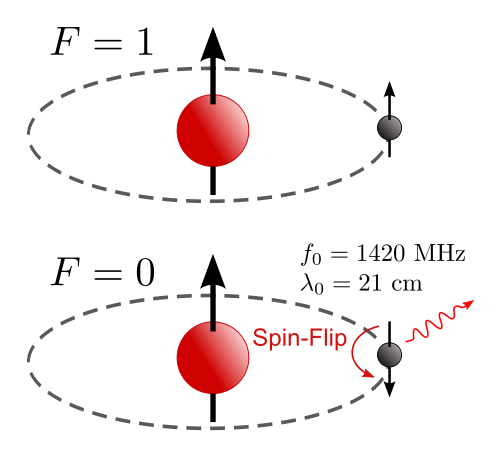
\includegraphics[width=4in]{chap0_intro/500px-Hydrogen-SpinFlip.svg.png}
	\caption[Diagram of the two Hydrogen ground states resulting from hyperfine splitting.]{Typical visualization of the two Hydrogen ground states resulting from the hyperfine splitting \citep{HydrogenSpinFlipGraphic}, where $F$ is the total angular momentum of the system, and the transition between the two states results in emission of a 21\,cm photon.}
	\label{fig:HydrogenSpinFlipGraphic}
\end{figure}

Finally, at higher order, the coupling of the proton and electron spins splits all states into those where the electron and proton spins are parallel, and those where they are antiparallel, as in Fig. \ref{fig:HydrogenSpinFlipGraphic}. The energy difference is much smaller than the differences between the $n=1,2,3$ states, and corresponds to emission or absorption of a low frequency radio photon with wavelength 21\,cm. In the upper (lower) state the spins are parallel (anti-parallel). Note that this disagrees with classical intuition, as when the spins are parallel, the magnetic dipole moments are antiparallel, and just as two antialigned magnets tend to attract, this state should actually have \textit{lower} energy. 

In response, is often remarked simply that quantum mechanics sometimes makes counterintuitive predictions, though \citet{griffiths82} argues that there is a more intuitive way to understand the situation. He observes that Fig. \ref{fig:HydrogenSpinFlipGraphic} misleadingly suggests that the electron is displaced from the proton, when in fact its spherical wavefunction encompasses it, and thus it is more correct to picture their magnetic moments as tiny current loops in the $xy$ plane (perpendicular to the proton spin). If both spins are aligned, then the current loops flow in opposite directions, and thus repel just like parallel wires with opposite currents, explaining which this is the higher energy state.

Lastly, note that in the upper state when the spins point in the same direction, the quantization of $z$ angular momentum makes this actually a spin triplet state, so there are three upper states and one lower state.

\subsection{21cm emission from the Dark Ages and Epoch of Reionization}

In this section I review theoretical calculacions of the observed 21\,cm brightness temperature of a neutral cloud in the intergalactic medium (IGM) during the Epoch of Reionization (EOR), mainly following \citet{PritchardLoebReview}, but filling in many missing details and background information where helpful. 

\subsubsection{Microscopic radiative transfer using Einstein A and B coefficients}

The Hydrogen atom is not a simple quantum mechanical system, and even less so taking into account fine and hyperfine structure, but fortunately in the cool, dilute intergalactic medium, the problem simplifies greatly. Essentially all hydrogen atoms are in the ground state at temperatures  $T<<10\text{eV}/k_B\sim10^5$K, which is always the case before the EOR when gas temperatures are $10-100$\,K, and after the EOR when they are $100-1000$\,K \citep{FurlanettoReview}. Thus only the hyperfine states are allowed, and we may regard such atoms at two level systems with an energy spacing of $\Delta E=hc/\lambda\approx6\mu$\,eV, where $\lambda=21$\,cm, and a three-fold degeneracy of the upper state. The four states are roughly equally populated as $T>>\Delta E/k_B =0.06$K, giving number densities of excited ($n=2$) and ground ($n=1$) state atoms as $n_2=\frac{3}{4}n_H$, and $n_1=\frac{1}{4}n_H$, where $n_H$ is the overall density of hydrogen atoms. Note that this $n$ indexes only the energy levels in this two level system, it is not the general $n$ used above to index the energy levels of hydrogen. Lastly, note that the spontaneous emission lifetime of the upper excited state is roughly $10^7$\,years.


MAYBE REPRODUCE A PLOT FROM FURLANETTO OR PRITCHARD SHOWING THE EVOLUTION OF ALL THREE TEMPERATURES

Before considering radiative transfer through the universe of 21\,cm emission from a hydrogen cloud at high redshift, we first comment on the different parts of this non thermodynamic equilibrium problem, and present the Einstein A and B coefficients we will use to synthesize them. The three temperatures in this problem are: (1) the hydrogen gas temperature, describing the root mean square velocities of the particles; (2), the spin temperature, defined as the temperature of an ensemble of two level atoms having the same ratio of excited to ground state atoms; and (3) the temperature of the cosmic microwave background, a blackbody radiation field which backlights our HI clouds during the EOR. 

Our problem is to calculate the emergent intensity of an HI cloud with optical depth $\tau$ backlit by the CMB. From standard radiative transfer theory, the answer is $I_\nu=I_0e^{-\tau}+S_\nu(1-e^{-\tau})$, however because our three temperatures are not the same, the source function $S_\nu\equiv j_\nu/\alpha_\nu$ does not in general equal a planck (i.e., blackbody) function\footnote{The planck function is given by $B_\nu(T)\propto\nu^3/(e^{h\nu/kT}-1)$} and we thus require a microscopic description of the radiation using the Einstein A and B coefficients.

Consider again our two level atom with number densities $n_2$ and $n_1$ in the excited and ground states, respectively. The Einstein coefficients are defined by:
\begin{eqnarray}
\text{\# spontaneous emissions per volume per time}&=&An_2 \nonumber\\
\text{\# stimulated emissions per volume per time}&=&B_{21}n_2u_\nu \nonumber\\
\text{\# absorptions per volume per time}&=&B_{12}n_1u_\nu 
\end{eqnarray}
Note that $A$ has units of $\text{s}^{-1}$, and the $B$'s have units of $\text{s}^{-1}(\text{energy density per frequency})^{-1}$. We can construct the unit of energy density per frequency as $h\nu/(c/\nu)^3/\nu$, thus on purely dimensional grounds we expect $A\approx B (h\nu^3/c^3)$, which is the correct relation from atomic physics up to a factor of $8\pi$. This demonstrates that spontaneous emission will be negligible at low radio frequencies. In that case, at equilibrium, the stimulated emission rate equals the absorption rate, giving $n_2B_{21}=n_1B_{12}\to g_2B_{21}=g_1B_{12}$.

What, then, is the source function of a system of such atoms? The radiative transfer equation is
\begin{equation}
\frac{dI_\nu}{ds}=j_\nu-\alpha_\nu I_\nu
\end{equation}
where $I_\nu$ is the specific intensity, with units of energy per area per solid angle per frequency per time. As the stimulated emission rate is proportional to the radiation density it makes sense to think of it contributing negatively to the absorption coefficient. So the emission coefficient is due solely to spontaneous emission, and has units of energy per volume per time per solid angle per frequency. Integrating over the spectral line, the energy emitted per volume per time per solid angle is:
\begin{equation}
\int j_\nu d\nu=\frac{1}{4\pi}h\nu n_2 A
\end{equation}
If we introduce a line shape $\phi(\nu-\nu_0)$ with $\int\phi(\nu-\nu_0)=1$, where $\nu_0$ is the center frequency of the spectral line, then we have:
\begin{equation}
\boxed{j_\nu=\frac{h\nu_0 n_2A\phi(\nu-\nu_0)}{4\pi}}
\end{equation}

Now consider a beam with intensity $I_\nu$ passing through the atoms. The energy density in the beam is $u_\nu=I_\nu/c$, so the energy absorbed from the beam per volume per time is $\int d\nu\int d\Omega\alpha_\nu I_\nu$, which can also be expressed as $\int d\nu h\nu_0\phi(\nu-\nu_0)(n_1B_{12}-n_2B_{21})I_\nu/c$, which gives:
\begin{equation}
\boxed{\alpha_\nu=\frac{h\nu_0\phi(\nu-\nu_0)(n_1B_{12}-n_2B_{21})}{c}}
\end{equation}

Then the source function is
\begin{equation}
\boxed{S_\nu=\frac{4}{4\pi}\frac{ n_2A}{n_1B_{12}-n_2B_{21}}}
\end{equation}
which is valid even if the atoms are not in thermodynamic equilibrium with the radiation field. 

\subsubsection{Brightness temperature of 21\,cm cloud at the EOR}

Now let us put the pieces of this calculation together and relate them to the observed emergent intensity of the CMB shining through an HI cloud during the EOR. As above, considering a radiation field with intensity $I_0$ behind a cloud of Hydrogen with optical depth $\tau$, the emergent intensity is $I_\nu=I_0e^{-\tau}+S_\nu(1-e^{-\tau})$. Cosmological redshift reduces the observed energy flux by $(1+z)$, and then reformulating the equation in terms of brightness temperatures and assuming $\tau<<1$ (because this is a very weak transition) gives
\begin{equation}
\delta T=\frac{T_s-T_\gamma(z)}{1+z}\tau 
\end{equation}
where $T_s$ is the brightness temperature of 21\,cm radiation from the gas, equal to the spin temperature of the gas\footnote{We can prove that the spin temperature equals the brightness temperature of the gas noting that $S_\nu=j_\nu/\alpha_\nu\propto A n_2/(n_1B_{12}-n_2B_{21})=\nu^2 T_s$, where the last equality uses $A\sim\nu^3B$, which is the rayleigh jeans relation with the spin temperature instead of the typical gas temperature}. Now we just need the optical depth through the cloud with size $ds$.

\begin{equation}
\tau=\int\alpha ds=\int\frac{h\nu}{c}\phi(\Delta\nu)(n_1B_{12}-n_2B_{21})ds
\end{equation}
Then using $g_1B_{12}=g_2B_{21}$, $g_2/g_1=3$, and $n_2/n_1=3e^{-h\nu/kT_s}$ gives

\begin{equation}
\tau=\int\frac{h\nu}{c}\phi(\Delta\nu)\frac{n_H}{4}B_{12}(1-e^{-h\nu/kT_s})ds
\end{equation}
using $n_H=n_1/4$, given that $T_s>>h\nu/k=0.1$K. Recall that $B$ has units of $A$ divided by energy density per frequency, giving $A\sim Bh\nu^3/c^3$, and to be precise there is an $8\pi$ here. Also taylor expand the exponential:

\begin{equation}
\tau=\phi(\Delta\nu)\frac{n_H}{4}\frac{Ac^2}{8\pi\nu}\frac{h}{kT_s}\Delta s
\end{equation}
Now use that photons travel on geodesics so we may replace $\Delta s=a(t)\Delta r$ by $c\Delta t=c\Delta z/(1+z)H(z)$, and also use that the line is doppler broadened by $\Delta\nu/\nu=v/c=H(z)\Delta s/c$, with $\phi(\Delta\nu)=1/\Delta \nu$, giving:

\begin{equation}
\tau=\frac{n_H}{4}\frac{Ac^2}{\nu}\frac{h}{8\pi kT}\frac{c}{H(z)\nu}
\end{equation}

\begin{equation}
\tau=\frac{T_s-T_\gamma(z)}{1+z}\frac{\Omega_b\rho_c(1+z)^3}{4}\frac{Ac^2}{8\pi\nu}\frac{h}{kT_s}\frac{c}{H_0\sqrt{\Omega_m}(1+z)^{3/2}\nu}
\end{equation}

\begin{eqnarray}
\delta T&=&\sqrt{1+z}\left(1-\frac{T_\gamma(z)}{T_s}\right)\frac{\Omega_b}{4}\frac{3H_0}{8\pi Gm_p}\frac{h}{8\pi k}\frac{c}  {\sqrt{\Omega_m}}\left(\frac{c^2A}{\nu^2}\right)\\
&=&10\text{mK}\left(\frac{1+z}{10}\right)^{1/2}\left(1-\frac{T_\gamma(z)}{T_s}\right)
\end{eqnarray}

where $T_s>>T_\gamma$ during reionization. This leads naturally into a discussion of the global history of the 21cm signal.

\subsubsection{History of the global 21\,cm signal}

SHOW A PLOT OF THE GLOBAL SIGNAL VS REDSHIFT

As we see above, the brightness temperature of the 21cm signal is determined by the spin temperature. That temperature is affected by three processes: collisional coupling with atoms and free electrons which couple the gas kinetic temperature to the spin temperature, radiative coupling to the CMB, and Ly$\alpha$-induced spin-flips via an excited state. 

$1100>z>200$
The universe is dense enough so that collisional coupling between atoms and residual free electrons holds $T_\text{gas}=T_\gamma=T_s$, and $\delta T=0$.

$200>z>50$
Now the gas is cooling adiabatically with $PV^\gamma=$const, with $\gamma=c_p/c_v=1+1/c_v$, and $c_v=f/2$. Note also that $TV^{\gamma-1}=$const, giving that $T\sim (1+z)^2$ for $f=3$ for a monotonic ideal gas. So the gas cools below the CMB temperature, and the spin temperature is still coupled to the gas temperature. Thus 21cm signal is now visible in absorption. This is the pristine cosmological signal, and is the long run focus of 21cm cosmology.

$50>z>z_\text{re}$
This is the epoch of heating at reionization, and the exact sequence of events is quite uncertain. The spin temperature gets heated far above the CMB temperature by the first luminous sources. 21cm fluctuations are sourced by some combinations of Ly$\alpha$ flux, density fluctuations, and neutral fraction fluctuations.  

$z_\text{re}>z$
Most of the universe is ionized, and 21cm signal is now only visible in large scale 21cm overdensities. 


\subsection{how to get from image cubes to power spectra (ie, unit transforms and FFTs)}

FT along freq to get fourier cube,
FT along u/v to get image cube 

optimal quadratic power spectrum estimators, essentially, generalized FT with arbitrary weighting


\section{A new generation of radio interferometers}

\subsection{The basics of radio interferometry and power spectrum estimation}

A radio interferometer is an array of separate antennas whose outputs are correlated with each other, and combined to form an image. It is ofter cheaper and easier to use such a ``synthetic aperture'' to improve resolution and collecting area than to simply build ever bigger single dish antennas. In this section I will review how we get from the individual antenna outputs to a sky image in a simple case.

\begin{figure}[h]
    \centering
    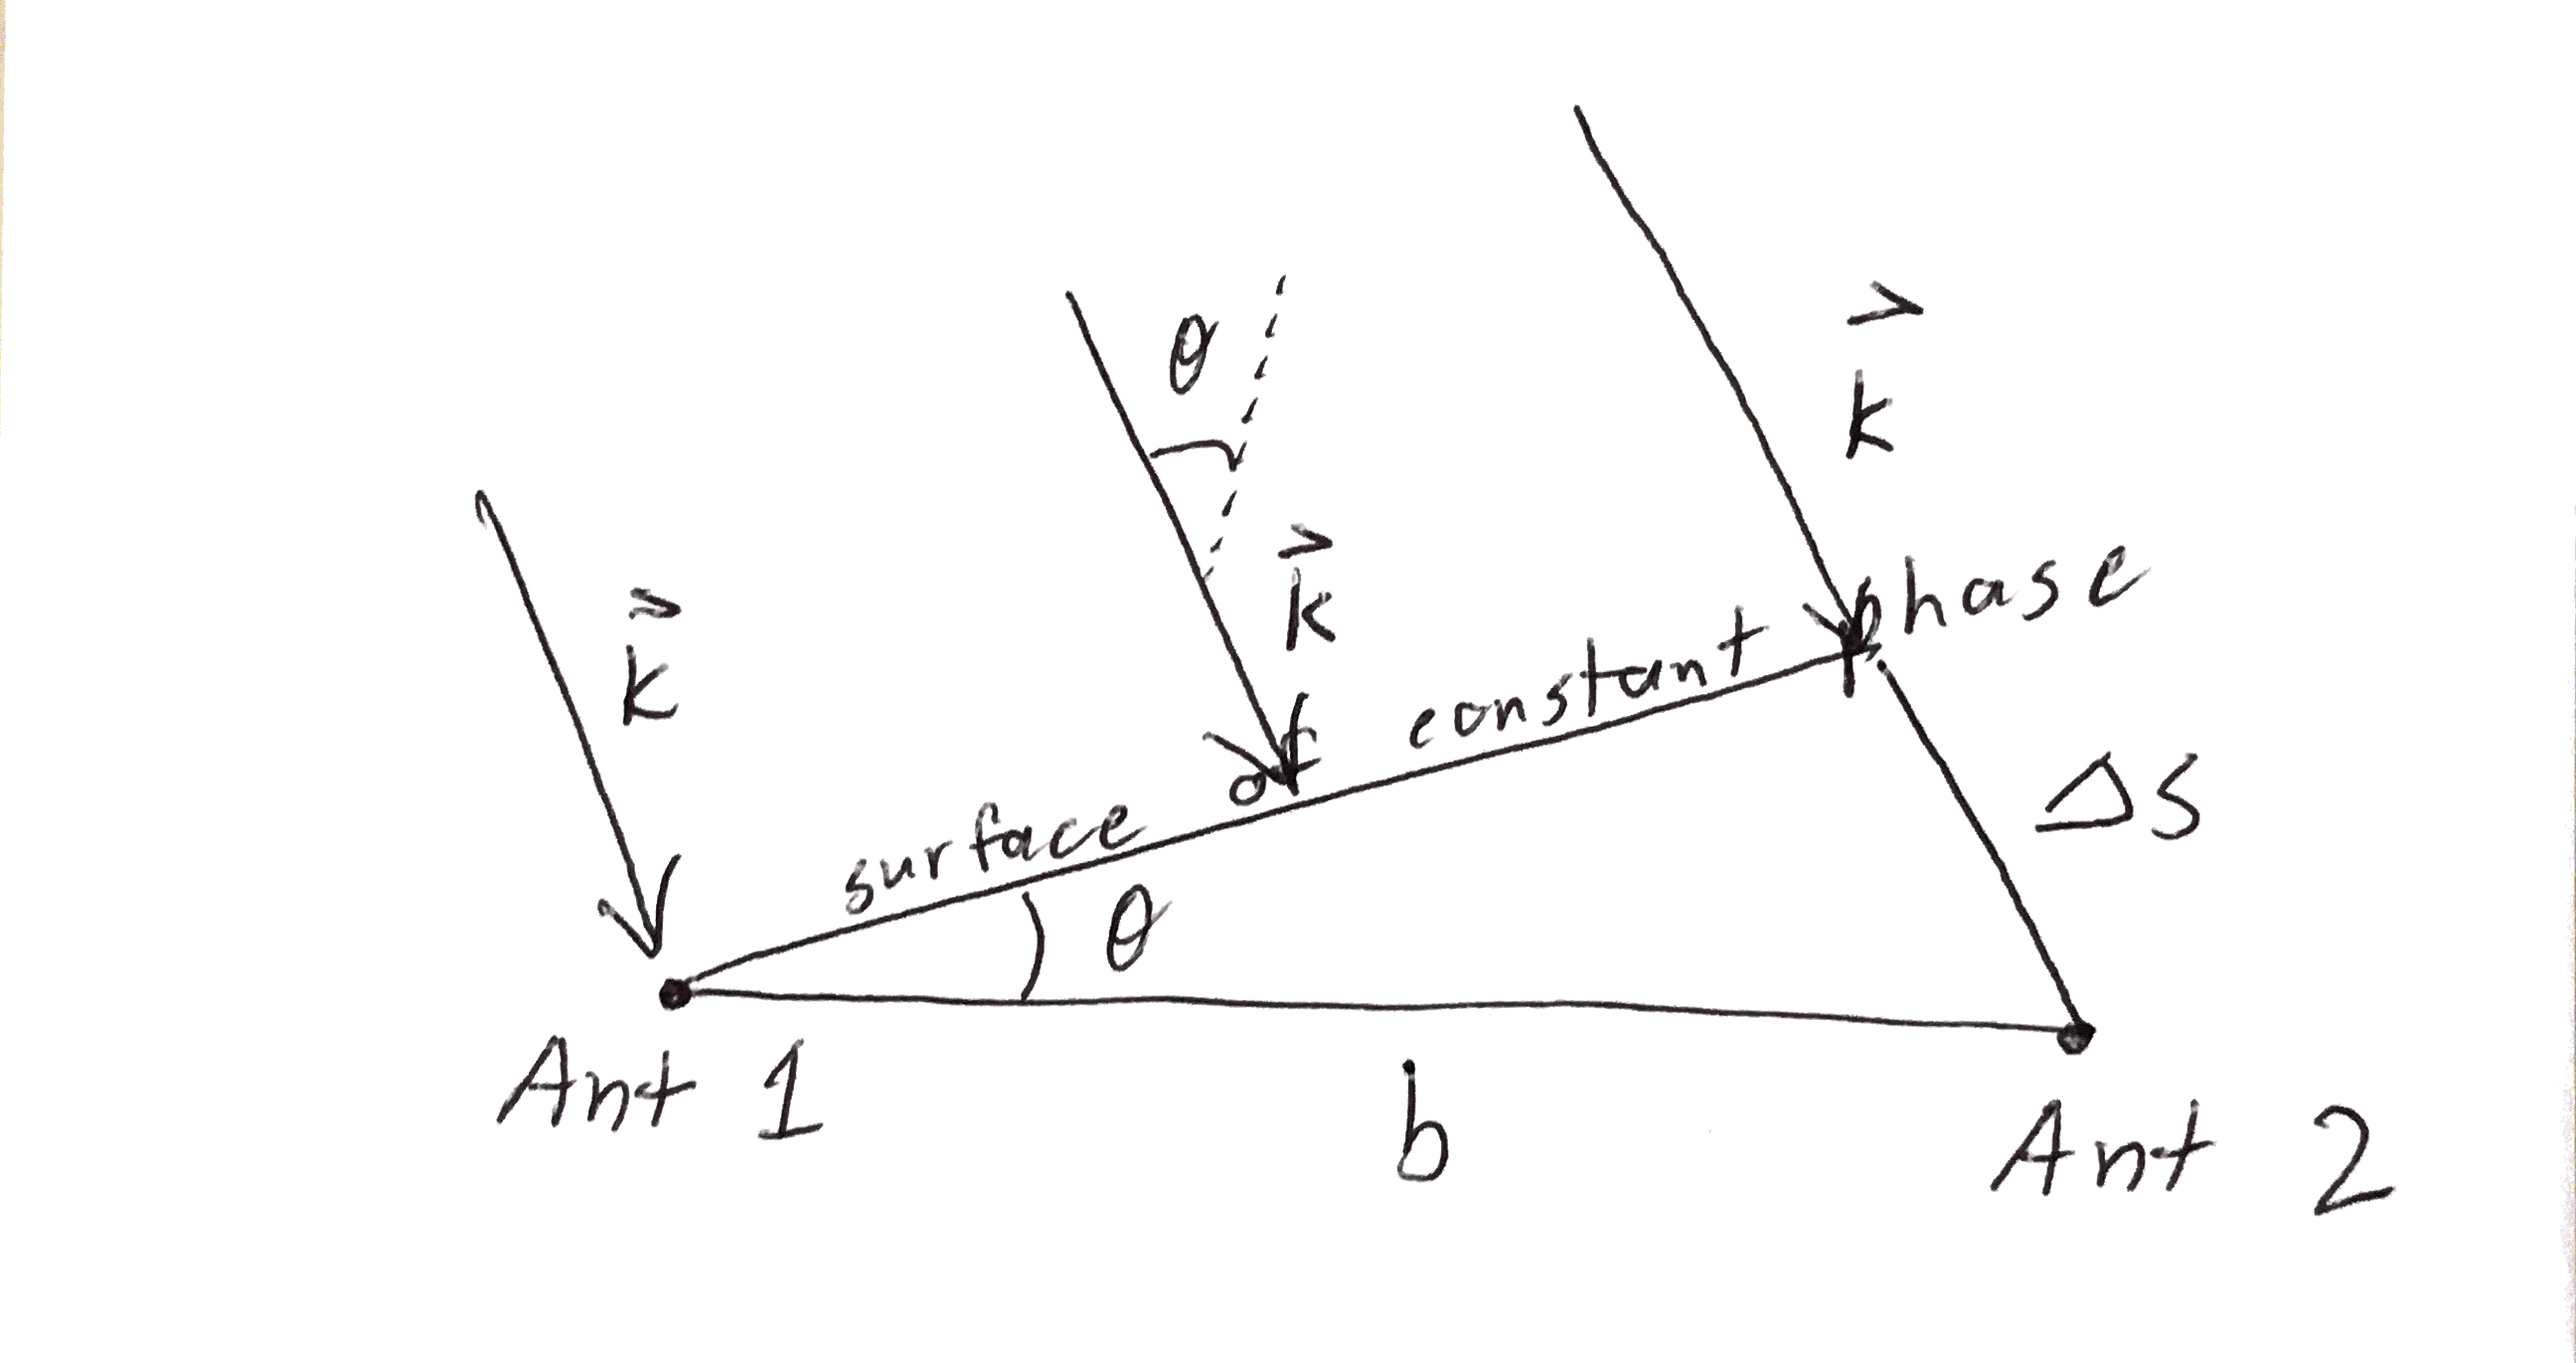
\includegraphics[width=0.95\textwidth]{chap0_intro/radio_interferometer_diagram.png}
    \caption[Diagram of a two element radio interferometer]{A single baseline (i.e., pair of antennas) displaced by $b$ on the ground receive radiation from a distant source at an angle $\theta$ from zenith. The source is distant enough that its surfaces of constant phase are planes which are orthogonal to $\vec{k}$, the wavevector of the radiation. The radiation arriving at Antenna 1 accumulates extra phase due to the path length difference $\Delta s$ compared to that arriving at Antenna 2.}
    \label{fig:radiointerferometerdiagram}
\end{figure}

Consider first a pair of antennas on the ground, known as a baseline, separated by $b$. Radiation arrives from a distant source at an angle $\theta$ from zenith. Note that after the surface of constant phase reaches Antenna 1, it propagates an extra path length of $\Delta s$ before reaching Antenna 2, equaling an extra phase of $\vec{k}\cdot \vec{\Delta s}=2\pi\sin b/\lambda$. Then the time averaged cross correlation between the voltages measured at antenna 1 and 2, known as the visibility $V_{12}$, is
\begin{equation}
	V_{12}\equiv\langle V_1(t)V_2^*(t)\rangle=\langle(V_0^* e^{i\omega t})(V_0e^{-i(\omega t-2\pi\sin b/\lambda)})\rangle \approx e^{2\pi i b\theta/\lambda}
\end{equation}
where we have used the small angle approximation. We can see that $b/\lambda$ and $\theta$ are fourier dual variables. If we can measure the visibility for many different $\vec{b}$ values, then we can grid them in $\vec{b}/\lambda$ space and take the fourier transform to get their representation in the $\theta$ space, also known as the sky image.

Suppose now that we have a pseudo random array of antennas with many different baseline lengths and orientations, described by the baseline sampling function $S(u,v)$, 
\begin{equation}
	 \mathcal{F}(S(u)Vs(u))=\mathcal{F}(\theta)\ast I(\theta)
\end{equation}
where $\mathcal{F}$ is the fourier transform operator and we have used the convolution theorem. Thus we recover the true image convolved with a point spread function, $\mathcal{F}(\theta)$, known in radio interferometry as the \textit{synthesized beam}. The synthesized beam is often non-compact and has significant sidelobes due to sparse $uv$ sampling, but can often be removed to quite high fidelity using iterative procedures like CLEAN \citep{hogbomclean}.

\begin{figure}[h]
    \centering
    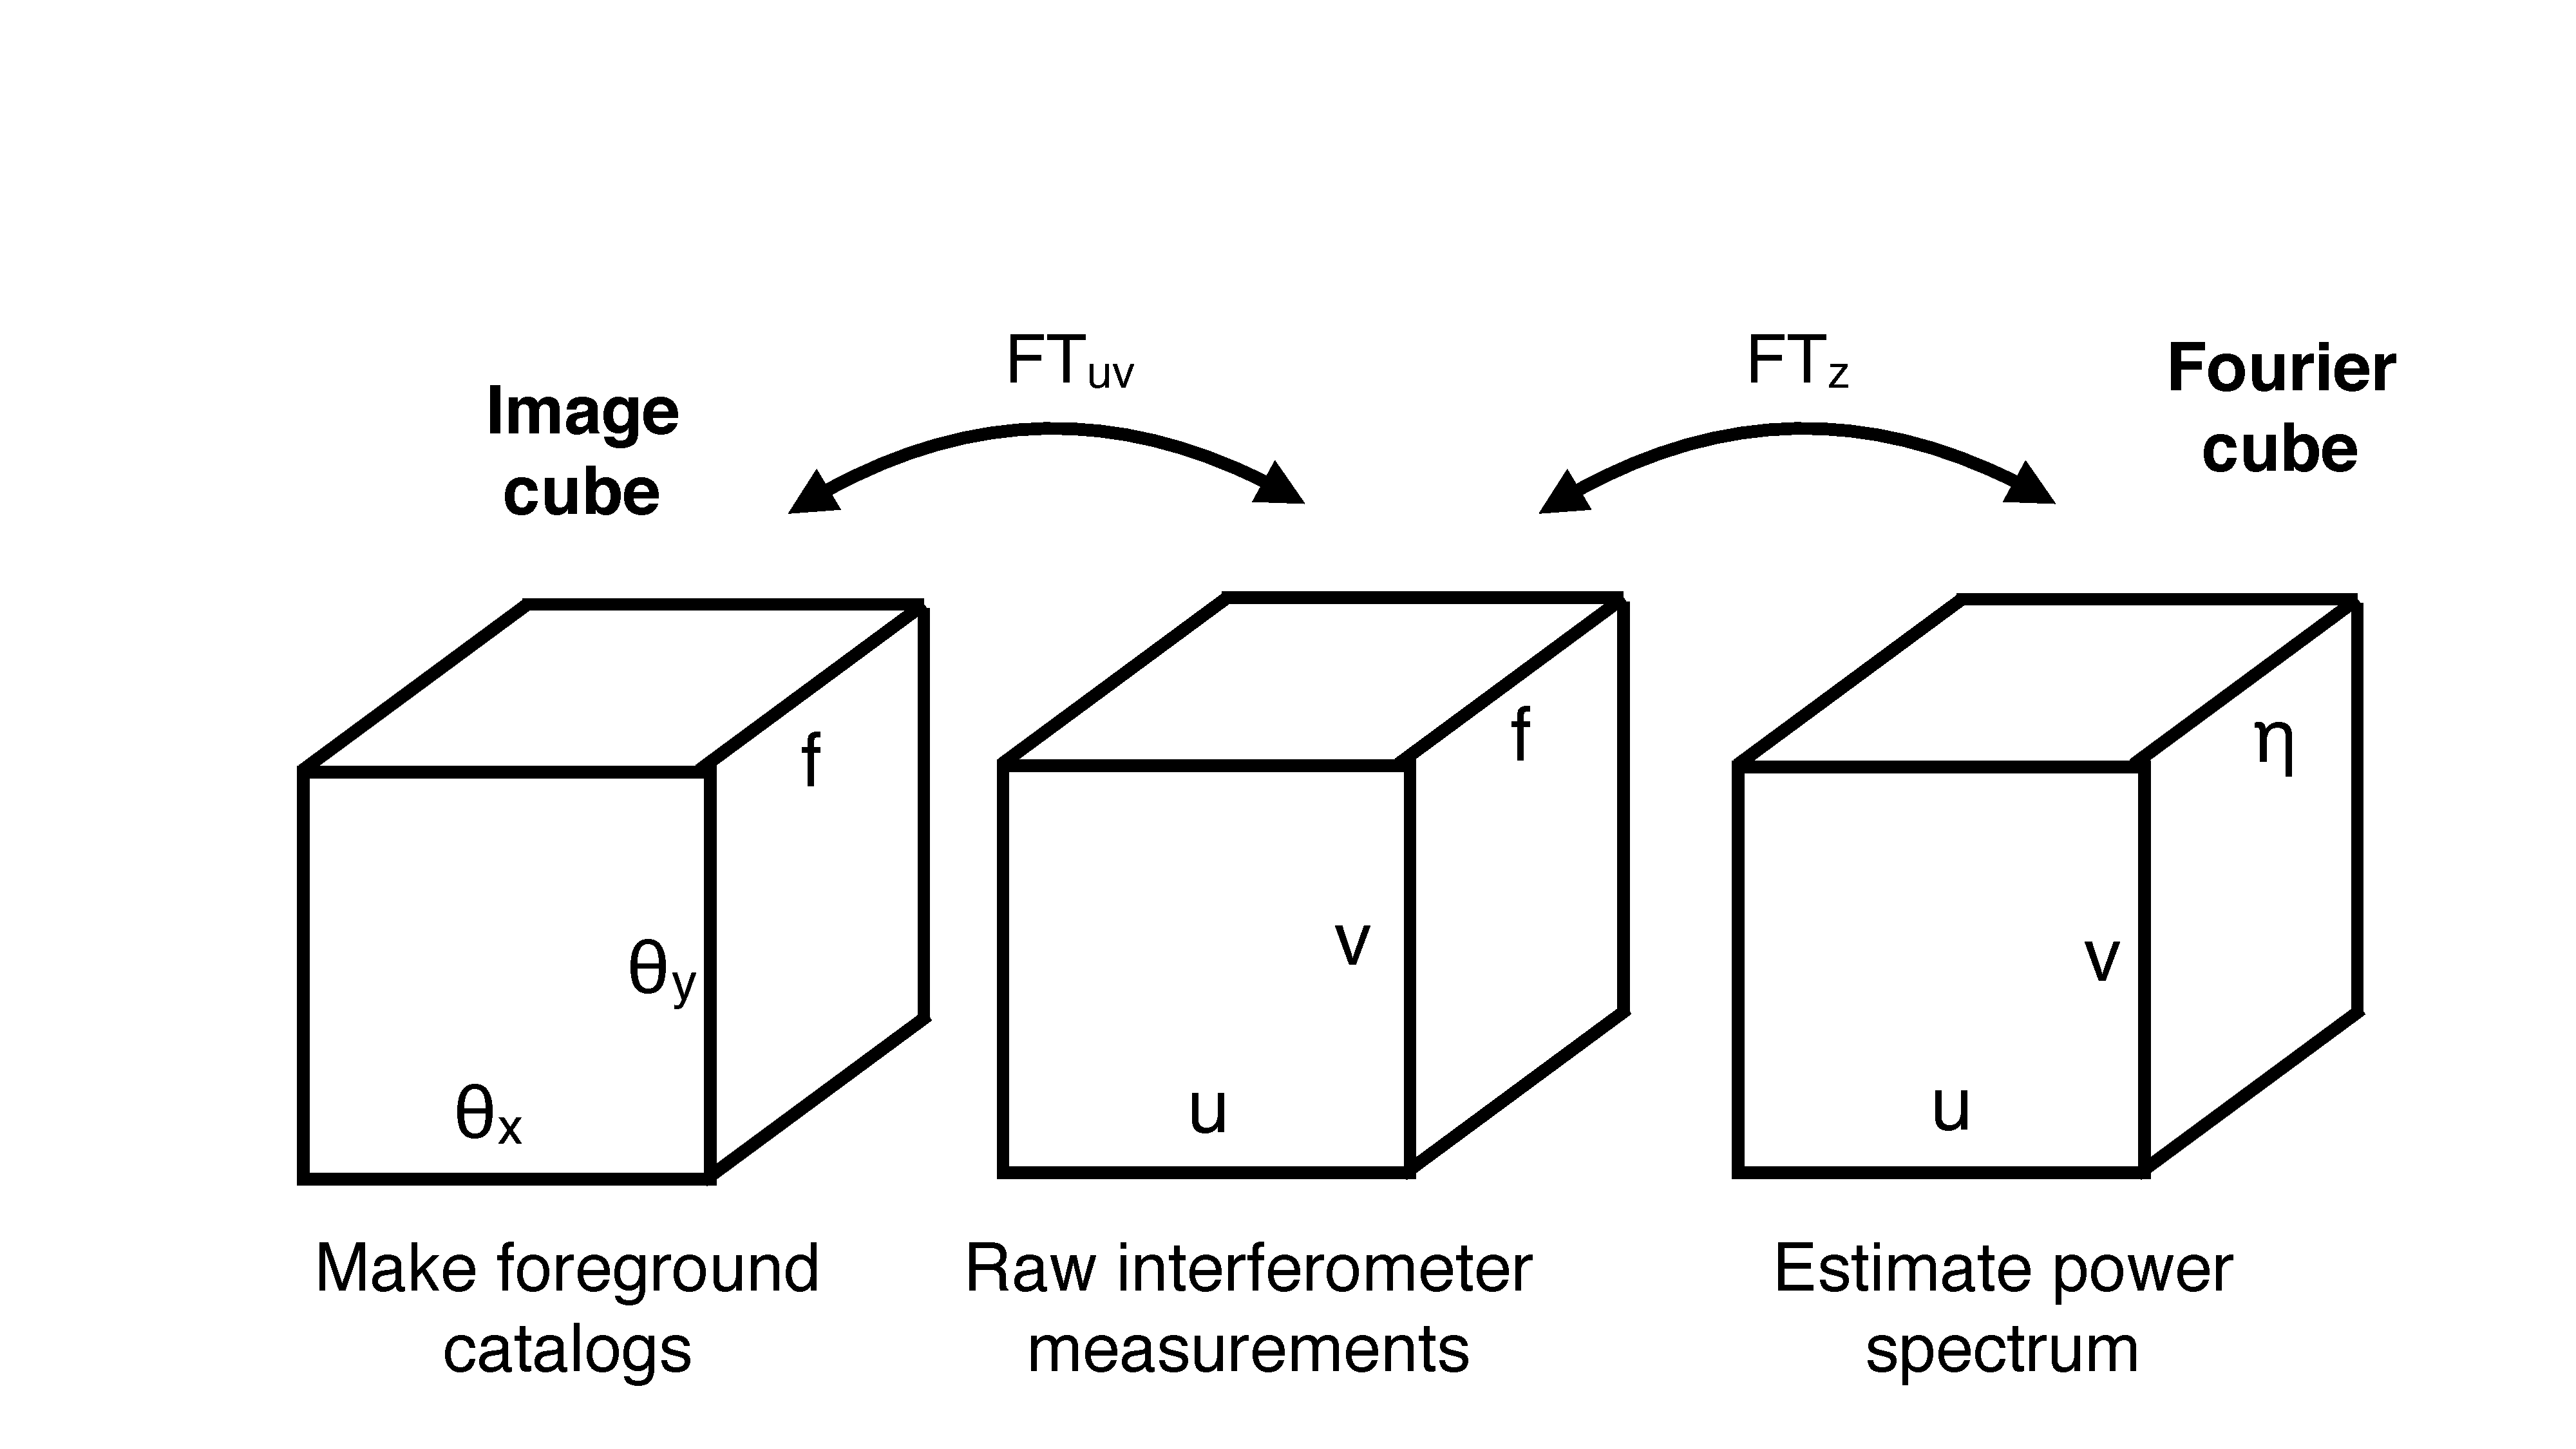
\includegraphics[width=0.8\textwidth]{chap0_intro/ifo_space.pdf}
    \caption[Representation of the relation between image space, fourier space, and interferometer space]{aoeuaoeu}
    \label{fig:ifospace}
\end{figure}




antennas, receivers, correlators (FX) vs omniscope
from baselines to images (FT)
random vs redundant arrays

\subsection{sensitivity requirements for EOR science and large D / small N regime}

3D sensitivity calculations, following beardsley's paper, using my math

\subsection{new gain/phase/primary beam calibration techniques/challenges}


\section{The problem of foregrounds}

\subsection{physics of galactic synchrotron}

Synchrotron radiation is the radiation observed from relativistic electrons spiraling around magnetic field lines in sources such as in cosmic ray electrons in our galaxy's magnetic field or  or radio galaxies which emit jets of charged particles, or ionized particles moving around pulsar magnetic fields in supernova remnants (ie, pulsar wind nebulae like the Crab). This radiation has a power law spectrum and is typically polarized (due to the preferred direction introduced by the magnetic field). 

First consider the effect of relativistic beaming. Radiation emitted isotropically in the frame of a particle moving relativistically is ``beamed'' in its direction of motion in the observer's frame. This is derived by Lorrentz transforming a photon's 4-momentum. Consider a photon emitted with angle $\theta$ from the $\hat{z}$ axis. Note $E=pc$.

\begin{equation}
\left(\begin{matrix}
E'\\
p_x'\\
p_y'
\end{matrix}\right)=
\left(\begin{matrix}
\gamma&\beta\gamma& 0\\
\beta\gamma&\gamma &0\\
0&0 &1
\end{matrix}\right)
\left(\begin{matrix}
E\\
p\cos\theta\\
p\sin\theta
\end{matrix}\right)=
\left(\begin{matrix}
E\gamma+p\cos\theta\beta\gamma\\
E\beta\gamma+p\cos\theta\gamma\\
p\sin\theta
\end{matrix}\right)
\end{equation}

So the photon, in our frame, was emitted at angle $\theta'$, given by:

\begin{equation}
\tan\theta'=\frac{\sin\theta}{\beta\gamma+\cos\theta\gamma}
\end{equation}

Consider radiation emitted at $\theta=\pi/2$ in the emitter's rest frame. If the object is highly relativistic, then $\beta\sim1$ and $\tan\theta'=1/\gamma$, giving $\theta'\sim1/\gamma$ Thus we may imagine relativistically moving emitters to be directing all their radiation out ahead of them into a cone with half angle $\theta'\sim1/\gamma$. 

Now consider an electron spiraling around a magnetic field line at the relativistic cyclotron frequency $\omega=eB/\gamma m$. See Figure \ref{fig:synchrotrondiagram}. 

\begin{figure}[h]
    \centering
    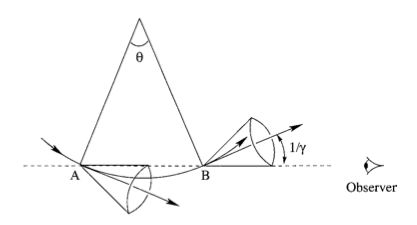
\includegraphics[width=0.75\textwidth]{chap0_intro/synchrotrondiagram.png}
    \caption[Diagram of electron gyration around a magnetic field line, resulting in synchrotron radiation.]{An electron gyrating around a magnetic field line, resulting in synchrotron radiation, from \citet{choudhuri2010astrophysics}.}
    \label{fig:synchrotrondiagram}
\end{figure}

Consider the time difference between radiation emitted at A and B. 

\begin{equation}
\Delta t=t_A-t_B=\frac{d}{c}-\left(\frac{\theta}{\omega}+\frac{d-R\theta}{c}\right)
\end{equation}
with $\theta\sim2/\gamma$ and $R=\omega v$. 

\begin{equation}
\Delta t = \frac{2m\gamma}{\gamma e B}-\frac{2mv\gamma}{\gamma eB c}=\frac{2m}{eB}(1-\beta)
\end{equation}
In the ultra-relativistic limit, $\beta\approx1-1/2\gamma^2$, giving $\Delta t=m/eB\gamma^2$. We thus expect the received radiation to have a strong frequency component at $f\sim1/\Delta t\to f\sim\gamma^2$. 

Then for charged particle motion in a uniform magnetic field, the Larmor formula for total power emitted picks up a factor of $\gamma^2$. Let the number of emitters with energy between $E$ and $E+dE$ be $E^{-p}dE$. Note that $E\propto\gamma$. These particles with energy $E$ radiate their power at $f\sim\gamma^2$ (see previous question), and there are $E^{-p}dE\sim f^{-p/2}df/f^{1/2}$, so the frequency spectrum is $f^{(-p+1)/2}df$. Many astrophysical particle distributions have $p\approx-2.5$, which gives $f(\nu)\propto\nu^{-0.75}$.

\subsection{extragalactic radio sources}


AGN and zoo of active galaxies

\subsection{foreground subtraction / avoidance}

subtraction requirements
the wedge (imaging wedge vs delay spectrum wedge)

\section{Completing the picture with cross correlations}

\subsection{examples of successful cross correlation results}
Tzu-Ching's result \citep{Chang2010,Masui2013}

\subsection{what could be learned from IR cross correlation}
more about the sources: pop2 vs pop3
topology of reionization, anticorrelation scale shows bubble size increasing over time

\citep{Heneka2016}
\citep{Fernandez2014,Silva2012,Mao2014,Lidz2008,Gong2014,Fernandez2013}

